%%%%%%%%%%%%%%%%%%%%%%%%%%%%%%%%%%%%%%%%
% datoteka diploma-FRI-vzorec.tex
%
%POZOR: ta verzija ne producira pdf datoteke v pdf/A formatu!!!
%namenjena je le za nalogo pri Diplomskem seminarju!
%
% vzorčna datoteka za pisanje diplomskega dela v formatu LaTeX
% na UL Fakulteti za računalništvo in informatiko
%
% na osnovi starejših verzij vkup spravil Franc Solina, maj 2021
% prvo verzijo je leta 2010 pripravil Gašper Fijavž
%
% za upravljanje z literaturo ta vezija uporablja BibLaTeX
%
% svetujemo uporabo Overleaf.com - na tej spletni implementaciji LaTeXa ta vzorec zagotovo pravilno deluje
%

\documentclass[a4paper,12pt,openright]{book}
%\documentclass[a4paper, 12pt, openright, draft]{book}  Nalogo preverite tudi z opcijo draft, ki pokaže, katere vrstice so predolge! Pozor, v draft opciji, se slike ne pokažejo!
 
\usepackage[utf8]{inputenc}   % omogoča uporabo slovenskih črk kodiranih v formatu UTF-8
\usepackage[slovene,english]{babel}    % naloži, med drugim, slovenske delilne vzorce
\usepackage[pdftex]{graphicx}  % omogoča vlaganje slik različnih formatov
\usepackage{fancyhdr}          % poskrbi, na primer, za glave strani
\usepackage{amssymb}           % dodatni matematični simboli
\usepackage{amsmath}           % eqref, npr.
\usepackage{hyperxmp}
\usepackage[hyphens]{url}
\usepackage{csquotes}
\usepackage[pdftex, colorlinks=true,
						citecolor=black, filecolor=black, 
						linkcolor=black, urlcolor=black,
						pdfproducer={LaTeX}, pdfcreator={LaTeX}]{hyperref}

\usepackage{color}
\usepackage{soul}

\usepackage{mathtools}

\usepackage[
backend=biber,
style=numeric,
sorting=nty,
]{biblatex}


\addbibresource{sources.bib} %Imports bibliography file


%%%%%%%%%%%%%%%%%%%%%%%%%%%%%%%%%%%%%%%%
%	DIPLOMA INFO
%%%%%%%%%%%%%%%%%%%%%%%%%%%%%%%%%%%%%%%%
\newcommand{\ttitle}{Vizualno sledenje na vgrajenih napravah}
\newcommand{\ttitleEn}{Visual tracking on embedded devices}
\newcommand{\tsubject}{\ttitle}
\newcommand{\tsubjectEn}{\ttitleEn}
\newcommand{\tauthor}{Nik Prinčič}
\newcommand{\tkeywords}{računalniški vid na vgrajenih napravah, DepthAI, vizualni sledilnik}
\newcommand{\tkeywordsEn}{embedded computer vision, DepthAI, visual tracker}

%%%%%%%%%%%%%%%%%%%%%%%%%%%%%%%%%%%%%%%%
%	HYPERREF SETUP
%%%%%%%%%%%%%%%%%%%%%%%%%%%%%%%%%%%%%%%%
\hypersetup{pdftitle={\ttitle}}
\hypersetup{pdfsubject=\ttitleEn}
\hypersetup{pdfauthor={\tauthor}}
\hypersetup{pdfkeywords=\tkeywordsEn}

%%%%%%%%%%%%%%%%%%%%%%%%%%%%%%%%%%%%%%%%
% postavitev strani
%%%%%%%%%%%%%%%%%%%%%%%%%%%%%%%%%%%%%%%%  

\addtolength{\marginparwidth}{-20pt} % robovi za tisk
\addtolength{\oddsidemargin}{40pt}
\addtolength{\evensidemargin}{-40pt}

\renewcommand{\baselinestretch}{1.3} % ustrezen razmik med vrsticami
\setlength{\headheight}{15pt}        % potreben prostor na vrhu
\renewcommand{\chaptermark}[1]%
{\markboth{\MakeUppercase{\thechapter.\ #1}}{}} \renewcommand{\sectionmark}[1]%
{\markright{\MakeUppercase{\thesection.\ #1}}} \renewcommand{\headrulewidth}{0.5pt} \renewcommand{\footrulewidth}{0pt}
\fancyhf{}
\fancyhead[LE,RO]{\sl \thepage} 
%\fancyhead[LO]{\sl \rightmark} \fancyhead[RE]{\sl \leftmark}
\fancyhead[RE]{\sc \tauthor}              % dodal Solina
\fancyhead[LO]{\sc Diplomska naloga}     % dodal Solina


\newcommand{\BibLaTeX}{{\sc Bib}\LaTeX}
\newcommand{\BibTeX}{{\sc Bib}\TeX}

%%%%%%%%%%%%%%%%%%%%%%%%%%%%%%%%%%%%%%%%
% naslovi
%%%%%%%%%%%%%%%%%%%%%%%%%%%%%%%%%%%%%%%%  

\newcommand{\autfont}{\Large}
\newcommand{\titfont}{\LARGE\bf}
\newcommand{\clearemptydoublepage}{\newpage{\pagestyle{empty}\cleardoublepage}}
\setcounter{tocdepth}{1}	      % globina kazala

%%%%%%%%%%%%%%%%%%%%%%%%%%%%%%%%%%%%%%%%
% konstrukti
%%%%%%%%%%%%%%%%%%%%%%%%%%%%%%%%%%%%%%%%  
\newtheorem{izrek}{Izrek}[chapter]
\newtheorem{trditev}{Trditev}[izrek]
\newenvironment{dokaz}{\emph{Dokaz.}\ }{\hspace{\fill}{$\Box$}}


%%%%%%%%%%%%%%%%%%%%%%%%%%%%%%%%%%%%%%%%%%%%%%%%%%%%%%%%%%%%%%%%%%%%%%%%%%%%%%%
%% PDF-A
%%%%%%%%%%%%%%%%%%%%%%%%%%%%%%%%%%%%%%%%%%%%%%%%%%%%%%%%%%%%%%%%%%%%%%%%%%%%%%%

%%%%%%%%%%%%%%%%%%%%%%%%%%%%%%%%%%%%%%%% 
% define medatata
%%%%%%%%%%%%%%%%%%%%%%%%%%%%%%%%%%%%%%%% 
\def\Title{\ttitle}
\def\Author{\tauthor, np0174@student.uni-lj.si}
\def\Subject{\ttitleEn}
\def\Keywords{\tkeywordsEn}

%%%%%%%%%%%%%%%%%%%%%%%%%%%%%%%%%%%%%%%% 
% \convertDate converts D:20080419103507+02'00' to 2008-04-19T10:35:07+02:00
%%%%%%%%%%%%%%%%%%%%%%%%%%%%%%%%%%%%%%%% 
\def\convertDate{%
    \getYear
}

{\catcode`\D=12
 \gdef\getYear D:#1#2#3#4{\edef\xYear{#1#2#3#4}\getMonth}
}
\def\getMonth#1#2{\edef\xMonth{#1#2}\getDay}
\def\getDay#1#2{\edef\xDay{#1#2}\getHour}
\def\getHour#1#2{\edef\xHour{#1#2}\getMin}
\def\getMin#1#2{\edef\xMin{#1#2}\getSec}
\def\getSec#1#2{\edef\xSec{#1#2}\getTZh}
\def\getTZh +#1#2{\edef\xTZh{#1#2}\getTZm}
\def\getTZm '#1#2'{%
    \edef\xTZm{#1#2}%
    \edef\convDate{\xYear-\xMonth-\xDay T\xHour:\xMin:\xSec+\xTZh:\xTZm}%
}

%\expandafter\convertDate\pdfcreationdate 

%%%%%%%%%%%%%%%%%%%%%%%%%%%%%%%%%%%%%%%%
% get pdftex version string
%%%%%%%%%%%%%%%%%%%%%%%%%%%%%%%%%%%%%%%% 
\newcount\countA
\countA=\pdftexversion
\advance \countA by -100
\def\pdftexVersionStr{pdfTeX-1.\the\countA.\pdftexrevision}


%%%%%%%%%%%%%%%%%%%%%%%%%%%%%%%%%%%%%%%%
% XMP data
%%%%%%%%%%%%%%%%%%%%%%%%%%%%%%%%%%%%%%%%  
\usepackage{xmpincl}
%\includexmp{pdfa-1b}

%%%%%%%%%%%%%%%%%%%%%%%%%%%%%%%%%%%%%%%%
% pdfInfo
%%%%%%%%%%%%%%%%%%%%%%%%%%%%%%%%%%%%%%%%  
\pdfinfo{%
    /Title    (\ttitle)
    /Author   (\tauthor, np0174@student.uni-lj.si)
    /Subject  (\ttitleEn)
    /Keywords (\tkeywordsEn)
    /ModDate  (\pdfcreationdate)
    /Trapped  /False
}

%%%%%%%%%%%%%%%%%%%%%%%%%%%%%%%%%%%%%%%%
% znaki za copyright stran
%%%%%%%%%%%%%%%%%%%%%%%%%%%%%%%%%%%%%%%%  

\newcommand{\CcImageCc}[1]{%
	\includegraphics[scale=#1]{./img/common/cc_cc_30.pdf}%
}
\newcommand{\CcImageBy}[1]{%
	\includegraphics[scale=#1]{./img/common/cc_by_30.pdf}%
}
\newcommand{\CcImageSa}[1]{%
	\includegraphics[scale=#1]{./img/common/cc_sa_30.pdf}%
}

%%%%%%%%%%%%%%%%%%%%%%%%%%%%%%%%%%%%%%%%%%%%%%%%%%%%%%%%%%%%%%%%%%%%%%%%%%%%%%%
%%%%%%%%%%%%%%%%%%%%%%%%%%%%%%%%%%%%%%%%%%%%%%%%%%%%%%%%%%%%%%%%%%%%%%%%%%%%%%%

\begin{document}
\selectlanguage{slovene}
\frontmatter
\setcounter{page}{1} %
\renewcommand{\thepage}{}       % preprečimo težave s številkami strani v kazalu

%%%%%%%%%%%%%%%%%%%%%%%%%%%%%%%%%%%%%%%%
%naslovnica
\thispagestyle{empty}%
\begin{center}
    {\large\sc Univerza v Ljubljani\\%
        %      Fakulteta za elektrotehniko\\% za študijski program Multimedija
        %      Fakulteta za upravo\\% za študijski program Upravna informatika
        Fakulteta za računalništvo in informatiko\\%
        %      Fakulteta za matematiko in fiziko\\% za študijski program Računalništvo in matematika
    }
    \vskip 10em%
        {\autfont \tauthor\par}%
        {\titfont \ttitle \par}%
        {\vskip 3em \textsc{DIPLOMSKO DELO\\[5mm]         % dodal Solina za ostale študijske programe
                VISOKOŠOLSKI STROKOVNI ŠTUDIJSKI PROGRAM\\ PRVE STOPNJE\\ RAČUNALNIŠTVO IN INFORMATIKA}\par}%
    % UNIVERZITETNI  ŠTUDIJSKI PROGRAM\\ PRVE STOPNJE\\ RAČUNALNIŠTVO IN INFORMATIKA}\par}%
    %    INTERDISCIPLINARNI UNIVERZITETNI\\ ŠTUDIJSKI PROGRAM PRVE STOPNJE\\ MULTIMEDIJA}\par}%
    %    INTERDISCIPLINARNI UNIVERZITETNI\\ ŠTUDIJSKI PROGRAM PRVE STOPNJE\\ UPRAVNA INFORMATIKA}\par}%
    %    INTERDISCIPLINARNI UNIVERZITETNI\\ ŠTUDIJSKI PROGRAM PRVE STOPNJE\\ RAČUNALNIŠTVO IN MATEMATIKA}\par}%
    \vfill\null%
    % izberite pravi habilitacijski naziv mentorja!
    {\large \textsc{Mentor}: doc. dr. Luka Čehovin Zajc \par}%
    % {\large \textsc{Somentor}:  viš. pred./doc./izr. prof./prof. dr.  Martin Krpan \par}%
    {\vskip 2em \large Ljubljana, \the\year \par}%
\end{center}
% prazna stran
%\clearemptydoublepage      
% izjava o licencah itd. se izpiše na hrbtni strani naslovnice

%%%%%%%%%%%%%%%%%%%%%%%%%%%%%%%%%%%%%%%%
%copyright stran
%%%%%%%%%%%%%%%%%%%%%%%%%%%%%%%%%%%%%%%%
\newpage
\thispagestyle{empty}

\vspace*{5cm}
{\small \noindent
    To delo je ponujeno pod licenco \textit{Creative Commons Priznanje avtorstva-Deljenje pod enakimi pogoji 2.5 Slovenija} (ali novej\v so razli\v cico).
    To pomeni, da se tako besedilo, slike, grafi in druge sestavine dela kot tudi rezultati diplomskega dela lahko prosto distribuirajo,
    reproducirajo, uporabljajo, priobčujejo javnosti in predelujejo, pod pogojem, da se jasno in vidno navede avtorja in naslov tega
    dela in da se v primeru spremembe, preoblikovanja ali uporabe tega dela v svojem delu, lahko distribuira predelava le pod
    licenco, ki je enaka tej.
    Podrobnosti licence so dostopne na spletni strani \href{http://creativecommons.si}{creativecommons.si} ali na Inštitutu za
    intelektualno lastnino, Streliška 1, 1000 Ljubljana.

    \vspace*{1cm}
    \begin{center}% 0.66 / 0.89 = 0.741573033707865
        \CcImageCc{0.741573033707865}\hspace*{1ex}\CcImageBy{1}\hspace*{1ex}\CcImageSa{1}%
    \end{center}
}

\vspace*{1cm}
{\small \noindent
    Izvorna koda diplomskega dela, njeni rezultati in v ta namen razvita programska oprema je ponujena pod licenco GNU General Public License,
    različica 3 (ali novejša). To pomeni, da se lahko prosto distribuira in/ali predeluje pod njenimi pogoji.
    Podrobnosti licence so dostopne na spletni strani \url{http://www.gnu.org/licenses/}.
}

\vfill
\begin{center}
    \ \\ \vfill
    {\em
        Besedilo je oblikovano z urejevalnikom besedil \LaTeX.}
\end{center}

% prazna stran
\clearemptydoublepage

%%%%%%%%%%%%%%%%%%%%%%%%%%%%%%%%%%%%%%%%
% stran 3 med uvodnimi listi
\thispagestyle{empty}
\
\vfill

\bigskip
\noindent\textbf{Kandidat:} Nik Prinčič\\
\noindent\textbf{Naslov:} Vizualno sledenje na vgrajenih napravah\\
% vstavite ustrezen naziv študijskega programa!
\noindent\textbf{Vrsta naloge:} Diplomska naloga na visokošolskem programu prve stopnje Računalništvo in informatika \\
% izberite pravi habilitacijski naziv mentorja!
\noindent\textbf{Mentor:} doc. dr. Luka Čehovin Zajc\\
% \noindent\textbf{Somentor:} isto kot za mentorja

\bigskip
\noindent\textbf{Opis:}\\
Besedilo teme diplomskega dela študent prepiše iz študijskega informacijskega sistema, kamor ga je vnesel mentor.
V nekaj stavkih bo opisal, kaj pričakuje od kandidatovega diplomskega dela.
Kaj so cilji, kakšne metode naj uporabi, morda bo zapisal tudi ključno literaturo.

\bigskip
\noindent\textbf{Title:} Visual tracking on embedded devices

\bigskip
\noindent\textbf{Description:}\\
opis diplome v angleščini

\vfill



\vspace{2cm}

% prazna stran
\clearemptydoublepage

% zahvala
\thispagestyle{empty}\mbox{}\vfill\null\it%
\noindent
Na tem mestu zapišite, komu se zahvaljujete za pomoč pri izdelavi diplomske naloge oziroma pri vašem študiju nasploh. Pazite, da ne boste koga pozabili. Utegnil vam bo zameriti. Temu se da izogniti tako, da celotno zahvalo izpustite.
\rm\normalfont

% prazna stran
\clearemptydoublepage

%%%%%%%%%%%%%%%%%%%%%%%%%%%%%%%%%%%%%%%%
% posvetilo, če sama zahvala ne zadošča :-)
\thispagestyle{empty}\mbox{}{\vskip0.20\textheight}\mbox{}\hfill\begin{minipage}{0.55\textwidth}%
    Svoji dragi Alenčici.
    \normalfont\end{minipage}

% prazna stran
\clearemptydoublepage


%%%%%%%%%%%%%%%%%%%%%%%%%%%%%%%%%%%%%%%%
% kazalo
\pagestyle{empty}
\def\thepage{}% preprečimo težave s številkami strani v kazalu
\tableofcontents{}


% prazna stran
\clearemptydoublepage

%%%%%%%%%%%%%%%%%%%%%%%%%%%%%%%%%%%%%%%%
% seznam kratic

\chapter*{Seznam uporabljenih kratic}

\noindent\begin{tabular}{p{0.11\textwidth}|p{.39\textwidth}|p{.39\textwidth}}    % po potrebi razširi prvo kolono tabele na račun drugih dveh!
    {\bf kratica} & {\bf angleško}               & {\bf slovensko}               \\ \hline
    {\bf AI}      & Artificial inteligence       & Umetna inteligenca            \\
    {\bf ANN}     & Artificial neural network    & Umetna nevronska mreža        \\
    {\bf BNN}     & Biological neural network    & Biološka nevronska mreža      \\
    {\bf DNN}     & Deep Neural Network          & Globoka nevronska mreža       \\
    {\bf CNN}     & Convolutional neural network & Konvolucijska nevronska mreža \\
    {\bf FPS}     & Frames per second            & Sličice na sekundo            \\
    {\bf OAK}     & OpenCV AI Kit                & OpenCV AI komplet             \\
    {\bf OAK}     & OpenCV AI Kit                & OpenCV AI komplet             \\
    {\bf BBOX}    & Bounding box                 & Omejitveni okvir              \\
    {\bf IoT}     & Internet of things           & Internet stvari               \\
    {\bf SOT}     & Single object tracking       & Sledenje posameznega objekta  \\
    {\bf MOT}     & Multiple object tracking     & Sledenje več objektom         \\
    {\bf VOT}     & Visual object tracking       & Vizualno sledenje             \\
    {\bf VPU}     & Visual processing unit       & Vizualna procesna enota       \\
    {\bf ROI}     & Region of interest           & Območje interesa              \\
    {\bf USB}     & Universal serial bus         & Univerzalno serijsko vodilo   \\
    {\bf PoE}     & Power over ethernet          & Napajanje preko etherneta     \\

    %  \dots & \dots & \dots \\
\end{tabular}


% prazna stran
\clearemptydoublepage

%%%%%%%%%%%%%%%%%%%%%%%%%%%%%%%%%%%%%%%%
% povzetek
\addcontentsline{toc}{chapter}{Povzetek}
\chapter*{Povzetek}

\noindent\textbf{Naslov:} \ttitle
\bigskip

\noindent\textbf{Avtor:} \tauthor
\bigskip

%\noindent\textbf{Povzetek:} 
\noindent V okviru diplomskega dela je bilo implementirano in ovrednoteno delovanje vizualnega sledilnika na vgrajeni napravi Luxonis OAK-1. Izbran je bil sledilnik STARK, spada v družino sledilnikov, ki jih sestavljajo globoke nevronske mreže. Bolj specifično sledilnik uporablja arhitekturo transformer, ki je trenutno uporabljena v vseh najboljših vizualnih sledilnikih. Sledilnik je bilo potrebno rahlo predelati ter ga prevesti v OpenVINO format, ki omogoča uporabno na vgrajeni napravi. Poleg tega je bilo potrebno zasnovati cevovod, po katerem se podatki na napravi pretakajo. Z vsem naštetim smo dosegli, da lahko vgrajena naprava izvaja vse potrebne funkcije popolnoma avtonomno, vse kar potrebuje od gostiteljskega sistema (npr. osebni računalnik) je začetni omejitveni okvir tarče \emph{(ang. bounding box)}, gostiteljskemu sistemu pa vrača vse naslednje omejitvene okvirje tarče. S tem smo dosegli to, da so performance sledenja neodvisne od gostiteljskega sistema.
\bigskip

\noindent\textbf{Ključne besede:} \tkeywords.
% prazna stran
\clearemptydoublepage

%%%%%%%%%%%%%%%%%%%%%%%%%%%%%%%%%%%%%%%%
% abstract
\selectlanguage{english}
\addcontentsline{toc}{chapter}{Abstract}
\chapter*{Abstract}

\noindent\textbf{Title:} \ttitleEn
\bigskip

\noindent\textbf{Author:} \tauthor
\bigskip

%\noindent\textbf{Abstract:} 
\noindent This sample document presents an approach to typesetting your BSc thesis using \LaTeX.
A proper abstract should contain around 100 words which makes this one way too short.
\bigskip

\noindent\textbf{Keywords:} \tkeywordsEn.
\selectlanguage{slovene}
% prazna stran
\clearemptydoublepage

%%%%%%%%%%%%%%%%%%%%%%%%%%%%%%%%%%%%%%%%
\mainmatter
\setcounter{page}{1}
\pagestyle{fancy}

\chapter{Uvod}
\section{Motivacija}
Računalniški vid je področje, ki se v zadnjih letih zelo hitro razvija. Z napredkov v razvoju avtonomnih sistemov, kot so avtonomni avtomobili, droni, roboti in še mnogi drugi, in vse večjem številu IoT naprav opremljenih s kamero, se vedno bolj pojavlja želja po uporabi modernih pristopov na majhnih, manj zmogljivih napravah. Področje računalniškega vida zavzema kar nekaj sklopov, v tem delu smo se osredotočili na vizualno sledenje, natančneje sledenju posameznega objekta \emph{(ang. single object tracking, VOT)}.

Vizualno sledenje je področje, ki se ukvarja z iskanjem in sledenjem objektov v videu. V tem delu smo se osredotočili na SOT, kjer je cilj slediti samo enemu objektu. Sledilniku je naprej potrebno podati omejevalni okvir tarče \emph{(ang. bounding box, BBOX)}, kateri želimo slediti, nato pa sledilnik na podlagi prostorske, pri najbolj modernih pa celo časovno-prostorske informacije sledi želeni tarči in nam za vsako naslednjo sličico vrne pripadajoč BBOX. V preteklosti so bil najbolj popularni tako imenovani klasični algoritmi (npr. KCF \cite{kcf}, MOSSE \cite{mosse}, ...), sedaj pa prevladujejo sledilniki, ki temeljijo na nevronskih mrežah. V zadnjih nekaj letih je upravičeno vedno bolj popularna arhitektura transformer \cite{attention_is_all_you_need}, ki je bila primarno razvita in uporabljena za razumevanje in generacijo teksta \emph{(ang. natural language processing, NLP)}, v zadnjih letih pa je bila adaptirana na vizualne sledilnike, kjer dosega odlične rezultate.

Da bi lahko zagotovili, dobre performance, pri manjši porabi energije, so se začele razvijati namenske procesorske enote VPU \emph{(ang. visual processing unit)}, ki so optimizirane za izvajanje nevronskih mrež in pospešeno izvajanje operacij na slikovnimi tokovi. V to družino procesorskih enot spada tudi čip, Intel Movidius Myriad X, ki je v osrčju uporabljen naprave v tem diplomskem delu.

V okviru te diplomske naloge smo se osredotočili na sledilnik STARK \cite{stark}, ter vgrajeno napravo Luxonis OAK-1. Cilj naloge je bil sledilnik prilagoditi uporabi na tej napravi, ga prevesti v potreben format, ter ga umestiti v cevovod. Cevovod je bilo potrebno tudi smiselno zasnovati, da v model pridejo pravilno oblikovani podatki.


\section{Pregled področja}
Na temo vizualnega sledenja vsako leto izide mnogo del. Skozi leta se neprestano spreminjajo pristopi, ki prinašajo najboljše rezultate. Različne trende in uspešnosti sledilnikov najbolje razberemo če pregledamo rezultate izziva VOT \emph{(ang. VOT challenge)} \cite{vot}, ki je eden najbolj uveljavljenih testov na področju vizualnega sledenja. VOT izziv vsako leto priredi evalvacijo novih sledilnikov. Sledilnike so v zadnji izvedbi, VOT2022 \cite{vot2022}, testirali na v sedmih različnih kategorijah. Glede na rezultate izziva v zadnjih nekaj letih, lahko opazimo porast v popularnosti in uspešnosti sledilnikov, ki uporabljajo arhitekturo transformer. Iz rezultatov VOT2022, objavljenih v \cite{vot2022}, lahko razberemo da 9 od najboljših 10 sledilnikov uporablja arhitekturo transformer, opazimo lahko tudi, da je kar 47\% vseh testiranih sledilnikov uporabilo to arhitekturo.

Na področju vizualnega sledenja na vgrajenih napravah, je bilo objavljenih že nekaj del, a nobeno od njih ni uporabilo sledilnika na osnovi arhitekture transformer. V članku \emph{Evaluation of Visual Tracking Algorithms for Embedded Devices}\cite{evaluation_of_visual_tracking_algorithms_for_embedded_devices} so primerjali performance med 5 klasičnimi algoritmi, teste so izvedli na napravi Raspberry Pi 3 B v1.2 in ugotovili, da z uporabo sledilnika KCF dobijo najboljše razmerje med hitrostjo in natančnostjo. V članku \emph{Real-Time Multiple Object Visual Tracking for Embedded GPU Systems}\cite{real_time_multiple_object_visual_tracking_for_embedded_gpu_systems}, so predstavili MOT \emph{(ang. multiple object tracking)} na napravi Nvidia Jetson TX2, kjer so uporabili več stopenjsko arhitekturo, detektor (YOLOv3 \cite{yolov3}) in sledilnik (KCF \cite{kcf}), in dobili dobre rezultate.


\section{Struktura diplomske naloge}
Diplomsko delo je razdeljeno v 5 delov. V poglavju 2 bomo opisali metodologijo, to zavzema hiter opis nevronskih mrež na splošno, arhitekture CNN in transformer ter predstavitev izbranega sledilnika. V poglavju 3 bomo opisali podrobnosti implementacije, kar vključuje opis uporabljene vgrajene naprave, prilagoditev modela ter njegovo pretvorbo v pravilen format, opis implementacije cevovoda in opis 4 različnih načinov delovanja, ki smo jih pripravili. V poglavju 4 bomo prestavili rezultate evalvacije, osredotočili se bomo na primerjavo med sledilnikom, ki je bil pognan samostojno na vgrajeni napravi proti tistemu, ki je pognan na osebnem računalniku. Predstavili bomo tudi rezultate primerjave med dvema načinoma delovanja, robni \emph{(ang. edge mode)} proti gostiteljskemu \emph{(ang. host mode)} načinu delovanja. V poglavju 5 je zaključek, ki povzema ugotovitve, ter predstavi možne izboljšave za nadaljnji razvoj.


\chapter{Metodologija}
\label{ch:1}
Ker je bil cilj dela, preizkusiti možnost uporabe enega izmed najsodobnejših vizualnih sledilnikov na vgrajeni napravi, ki temelji na nevronskih mrežah, bomo v tem poglavju predstavili delovanje nevronskih mrež, arhitekture CNN in transformer in opisali izbrani sledilnik.

\section{Umetne nevronske mreže}
Umetne nevronske mreže \emph{(ang. Artificial Neural Network, ANN)} so vrsta modelov strojnega učenja, ki posnemajo delovanje bioloških nevronskih mrež \emph{(ang. Biological Neural Network, BNN)}. Sestavljene so iz množice umetnih nevronov, ki so med seboj povezani z uteženimi povezavami in združeni v sloje. Sloje delimo na tri vrste - vhodni sloj \emph{(ang. input layer)}, skrite sloje \emph{(ang. hidden layers)} in izhodni sloj \emph{(ang. output layer)}. Mreže z več kot enim skritim slojem imenujemo globoke nevronske mreže \emph{(ang. Deep Neural Network, DNN)} ostale pa smatramo kot plitve nevronske mreže. Na sliki \ref{img:nn_vs_dnn} je prikazana primerjava zgradbe med plitvo nevronsko mrežo (levo) in globoko nevronsko mrežo (desno).

\begin{figure}[htb]
    \begin{center}
        \includegraphics[width=0.8\textwidth]{img/nn_vs_dnn.png}
    \end{center}
    \caption{Primerjava zgradbe NN in DNN \cite{nn_vs_dnn}.}
    \label{img:nn_vs_dnn}
\end{figure}

Najpogosteje se za učenje nevronskih mrež uporablja algoritem vzvratnega razširjanja \emph{(ang. backpropagation)}. Algoritem se izvaja v več iteracijah, pri katerih se s pomočjo kriterijske funkcije izračuna napaka, ki je razlika med želenim izhodom in dejanskim izhodom. Napako uporabimo za izračun gradienta, ki nam pove, kako moramo spremeniti vrednost uteži, da se napaka zmanjša. Kriterijsko funkcijo morem pravilno izbrati glede na vrsto problema, ki ga želimo rešiti. Za reševanje regresijskih problemov se najpogosteje uporablja srednjo kvadratno napako \emph{(ang. Mean Squared Error, MSE)}, za klasifikacijske probleme pa najpogosteje kategorično križno entropijo \emph{(ang. Categorical Cross-Entropy)} ali pa binarno križno entropijo \emph{(ang. Binary Cross-Entropy)}. Za iskanje optimalnih vrednosti uteži se uporabljajo različni optimizacijski algoritmi, ki na podlagi gradientnega spusta \emph{(ang. gradient descent)} iščejo minimum kriterijske funkcije. Med njimi sta najbolj znan stohastični gradientni spust \emph{(ang. Stochastic Gradient Descent, SGD)} in Adam \emph{(ang. Adaptive Moment Estimation)}.

\section{Konvolucijske nevronske mreže}
Konvolucijske nevronske mreže \emph{(ang. Convolutional Neural Network)}, so vrsta umetnih nevronski mrež, ki se pogosto uporablja v nalogah računalniškega vida, kot so prepoznavanje objektov, klasifikacija slik, detekcija obrazov in drugo. CNN modeli so tipično sestavljeni iz več ponovitev konvolucijskih slojev \emph{(ang. convolutional layers)} in združevalnih slojev \emph{(ang. pooling layers)}. Za zadnjim združevalnim slojem najpogosteje sledi nekaj polno-povezanih slojev. Poenostavljena arhitektura konvolucijske nevronske mreže je prikazana na sliki \ref{img:cnn}.


\begin{figure}[htb]
    \begin{center}
        \includegraphics[width=0.8\textwidth]{img/cnn.jpg}
    \end{center}
    \caption{Poenostavljena arhitektura konvolucijkse nevronske mreže \cite{cnn}.}
    \label{img:cnn}
\end{figure}

Namen konvolucijskih slojev je pridobivanje značilk \emph{(ang. feature extraction)}, namen združevalnih slojev je zmanjševanje dimenzionalnosti podatkov, polno-povezani sloji pa so namenjeni preslikovanju pridobljenih značilk v končni izhod.

Konvolucijski sloji delujejo na principu matematične operacije konvolucije, ki je definirana na dveh funkcijah. Rezultat konvolucije nam pove, kako oblika ene spremeni obliko druge. Definirana je z enačbo:
\begin{equation}
    (f*g)(t)=\int_{\tau=-\inf}^{\inf}f(\tau)g(t-\tau)d\tau
    \label{eq:1}
\end{equation}

Kjer je \emph{f} predstavlja vhodno funkcijo, \emph{g} pa jedro konvolucije. Ker se pri obdelavi digitalnih podatkov pogosto uporablja diskretna konvolucija, z enačbo \ref{eq:1} spremenjena v:
\begin{equation}
    (f*g)[t]=\sum_{k=-\inf}^{\inf}f[k]g[n - k]
    \label{eq:2}
\end{equation}

\section{Arhitektura transformer}
Transformer je arhitektura nevronske mreže, ki temelji na mehanizmu pozornosti, ki je bil predstavljen leta 2017 v članku \emph{Attention is all you need} \cite{attention_is_all_you_need}. Primarno je bila arhitektur razvita za naloge procesiranja naravnega jezika \emph{(Natural language processing, NLP)}, sejda pa postaja popularna tudi v drugih domenah strojnega učenja, med drugim tudi v računalniškem vidu. Osnovna arhitektura, kji je bila predstavljena v \cite{attention_is_all_you_need}, vključuje kodirni \emph{(ang. encoder)} in dekodirni modul \emph{(ang. decoder)}. Kodirnik je sestavljen iz dveh podslojev, dekodirnik pa iz treh.

\subsection{Mehanizem pozornosti}
Mehanizem pozornosti deluje na podlagi ključev \emph{(ang. key, K)}, poizvedb \emph{(ang. query, Q)} in vrednosti \emph{(ang. value, V)}. Mehanizem iz matrike ključev in matrike poizvedb izračuna matriko pozornosti. Z matričnim množenjem matrike pozornosti in matrike vrednosti dobimo linearno kombinacijo vrednosti, ki predstavljajo izhod. Razlikujemo med samo-pozornostjo in med-pozornostjo. O samo-pozornosti govorim, ko vse tri vhodne parametre dobimo iz iste množice podatkov, pri med-pozornosti pa poizvedbe pridobimo iz ene množice podatkov, ključe in vrednosti pa iz druge.

Vhodne vektorje $ x_i, x_{i+1},..., x_{n} $ združimo v matriko $ X_{n \times d_m} $, kjer $ d_m $ predstavlja dimenzionalnost modela. Naučene parametre pa predstavljajo matrike $ W^Q_{d_m \times d_m} $, $ W^K_{d_m \times d_m} $ in $ W^V_{n \times d_m} $. Iz navedenih matrik lahko izračunamo

\begin{equation}
    \begin{split}
        Q = XW^Q, \\
        K = XW^K, \\
        V = XW^V, \\
    \end{split}
    \label{eq:3}
\end{equation}

Matrika pozornosti je definirana z enačbo:
\begin{equation}
    A(Q, K, V) = \text{softmax}(\frac{QK^T}{\sqrt{d_m}})V
    \label{eq:4}
\end{equation}

kjer funkcija \emph{softmax} spremeni vektor \emph{n} realnih števil v vektor verjetnostne porazdelitve.

Iz \ref{eq:3} in \ref{eq:4} lahko izračunamo končno izhodno vrednost mehanizma

\begin{equation}
    S = AV,
    \label{eq:5}
\end{equation}

na sliki \ref{img:attention} je potek izračuna prikazan v obliki diagrama.


Ko se mehanizem pozornosti uporabi v dekodirnem modulu je potrebno določen del podatkov skriti. Bolj natančno, modelu je treba preprečiti, z podatki, ki jih še ni napovedal.


\begin{figure}[htb]
    \begin{center}
        \includegraphics[width=0.3\textwidth]{img/attention.png}
    \end{center}
    \caption{Diagram izračuna pozornosti \cite{attention_is_all_you_need}.}
    \label{img:attention}
\end{figure}


\subsection{Več-glava pozornost}
Da bi model lahko zajel več lastnosti vhodnih podatkov je potrebno mehanizem pozornosti nadgraditi. Več-glava pozornost vzporedno izračuna več ločenih pozornosti (glav) in jih združi v končni rezultat. Vsaka glava se osredotoči na eno lastnost podatkov. Vsaka glava $ i $ ima svoje matrike naučenih uteži, končni rezultat pa se pridobi s strnitvijo posameznih matrik pozornosti. Na sliki \ref{img:mha} je prikazan diagram poteka več-glave pozornosti.

\begin{figure}[htb]
    \begin{center}
        \includegraphics[width=0.3\textwidth]{img/mha.png}
    \end{center}
    \caption{Diagram izračuna več-glave pozornosti \cite{attention_is_all_you_need}.}
    \label{img:mha}
\end{figure}


\subsection{Vhodna vdelava in pozicijsko kodiranje}
Preden vhodni podatki prispejo do kodirnega bloka jih je potrebno najprej pravilno predelati. Za ta namen se uporablja vdelava vhodnega niza v $ d_m $ dimenzionalni latentni prostor \emph{(ang. embedding space)}. Vhodna vdelava \emph{(ang. input embedding)} vhodne besede pretvori v vektorje, s tem model pridobi informacijo o pomenu posamezne besede. Pozicijsko kodiranje \emph{(ang. positional encoding)} pa modelu poda informacijo o vrstnem redu besed v nizu. Da bi se izognili velikim vrednostim v pozicijskem kodiranju, se za kodiranje uporabljata sledeči funkciji \ref{eq:7}

\begin{equation}
    \begin{split}
        PE(pos, 2i) = sin(pos/10000^{2i/d_m}) \\
        PE(pos, 2i+1) = cos(pos/10000^{2i/d_m})
    \end{split}
    \label{eq:7}
\end{equation}

v enačbi \ref{eq:7} predstavlja $ pos $ pozicijo besede v nizu, $ i $ pa dimenzijo kodiranja, kar pomeni da ima vsaka dimenzija pozicijskega kodiranja pripadajočo sinusoidno vrednost.


Informacijo o pomenu in poziciji posamezne besede združimo tako, da matriki seštejemo.

\subsection{Kodirni modul}
Kodirni modul ali kodirnik je sestavljen iz $ N $ identičnih slojev, ki so sestavljeni iz dveh pod-slojev. Prvi pod sloj je več glava pozornost \emph{(ang. multi-headed attention)} in polno povezane usmerjene nevronske mreže \emph{(ang. Feedforward neural network, FFN)}.

\begin{figure}[htb]
    \begin{center}
        \includegraphics[width=0.3\textwidth]{img/encoder.png}
    \end{center}
    \caption{Diagram kodrinega modula \cite{attention_is_all_you_need}.}
    \label{img:encoder}
\end{figure}


\subsection{Dekodirni modul}
Dekodirni modul ali dekodirnik je sestavljen iz $ N $ identičnih slojev, ki so sestavljeni iz treh pod-slojev. Prvi pod sloj je več glava pozornost z možnostjo maskiranja vhodnih podatkov. Drugi pod sloj je več glava pozornost, tretji sloj pa predstavlja polno povezana nevronska mreža.


\begin{figure}[htb]
    \begin{center}
        \includegraphics[width=0.3\textwidth]{img/decoder.png}
    \end{center}
    \caption{Diagram dekodirnega modula \cite{attention_is_all_you_need}.}
    \label{img:decoder}
\end{figure}

\section{Model STARK}
\label{sec:stark}
Model STARK \cite{stark} spada v družino SOT \emph{(ang. single object tracking)} sledilnikov. Primarno je sestavljen iz dveh arhitektur, konvolucijskih nevronskih mrež in arhitekture transformer, ki je bila prilagojena za vizualne sledilnike. Navdih za njegov nastanek je bil predhodni model za detekcijo DETER \cite{deter}. Ena od novosti, ki so jo uvedli v tem modelu je uporaba časovne in prostorske komponente \emph{STARK\_ST}. Prostorska komponenta vsebuje informacijo o izgledu objekta, kateremu sledi. Časovna komponenta pa nosi informacijo o spremembi pozicije objekta skozi čas.
Arhitektura, ki so jo predlagali vsebuje tri ključne elemente: kodirni modul, dekodirni modul in napovedovalno glavo \emph{(ang. predictio head)}. Model kot vhod prejme trenutno sliko, začetno matrico \emph{(ang. template)} in dinamično matrico, ki se skozi čas dinamično posodablja. Z uporabo dinamična matrice, ki se skozi čas posodablja, lahko model zajame prostorsko in časovno informacijo o objektu, ki mu sledimo.

Prednost tega sledilnika je v tem, da ne potrebuje kompleksne predobdelave \emph{(ang. preprocessing)} vhodnih podatkov in naknadne obdelave \emph{(ang. postprocessing)} izhoda. Ob inicializaciji prejem kot vhod sliko in omejitveni okvir tarče. Na podlagi teh dveh vhodnih podatkov se najprej iz celotne vhodne slike izreže iskalno območje \emph{(ang. search area)}, ki se uporabi za izračun matrice. Ob vsaki naslednji sličici, pa so vhodni podatki iskalno območje izrezano iz vhodne slike, začetna matrica in dinamična matrica, sledilnik pa vrne izračunani omejitveni okvir.

\subsection{Arhitektura modela stark}
V tem delu smo zaradi manjše procesorske in prostorske zahtevnosti uporabili, različico modela STARK, ki uporablja samo prostorsko komponento \emph{STARK\_S}. V nadaljevanju bomo predstavili delovanje in arhitekturo modela.

Arhitekturo modela lahko razdelimo na tri glavne dele: \emph{(1)} konvolucijska hrbtenica \emph{(ang. convolutional backbone)}, \emph{(2)} kodirni-dekodirni transformer in predikcijsko glavo za omejitveni okvir \emph{(ang. bounding box prediction head)}. V nadaljevanju bomo predstavili vsakega od teh delov.


\begin{figure}[htb]
    \begin{center}
        \includegraphics[width=0.8\textwidth]{img/stark.png}
    \end{center}
    \caption{Diagram arhitekture modela STARK\_S \cite{attention_is_all_you_need}.}
    \label{img:stark}
\end{figure}

\subsubsection{Konvolucijska hrbtenica}
Konvolucijsko hrbtenico sestavlja model ResNet \cite{resnet}, kateremu so odstranili zadnjo sekcijo in polno povezane sloje. Kot vhod prejme hrbtenica začetno matrico $ z \in \mathbb{R}^{3 \times H_z \times W_z} $ in iskalno območje $ x \in \mathbb{R}^{3 \times H_x \times W_x} $. Po prehodu čez hrbtenico dobimo dve matrici značilk
$ f_z \in \mathbb{R}^{C \times \frac{H_z}{s} \times \frac{W_z}{s}} $ in $ f_x \in \mathbb{R}^{C \times \frac{H_x}{s} \times \frac{W_x}{s}} $.

\subsection{Kodirnik}
Na matriki značilk, ki jo izračuna hrbtenica, je najprej potrebno izvesti predobdelavo. Predobdelava vključuje sloj z ozkim grlom \emph{(ang. bottleneck layer)}, ki matrikam zmanjša prostorsko dimenzionalnost iz $ C $ na $ d $. Nato je matriki potrebno sploščiti in združiti vzdolž prostorske dimenzije. Rezultat prejšnjih dveh operaciji proizvede sekvenco značilk dolžine $ \frac{H_z}{s}\frac{W_z}{s} + \frac{H_x}{s}\frac{W_x}{s} $ in dimenzionalnosti $ d $. Novo pridobljeni sekvenci značilk prištejemo vrednosti pozicijskega kodiranja vhoda. Ta sekvenco značilk je vhod za kodirni modul. Kodirni modul je sestavljen iz $ N $ identičnih slojev. Sloji so sestavljeni iz več-glave samo-pozornosti in FFN. Kodirni modul zajame odvisnosti med vsemi značilkami v vhodni sekvenci in s tem omogoča modelu, da se nauči o diskirminativnih značilkah, katere se uporabijo za lokalizacijo objekta.

\subsection{Dekodirnik}
Dekodirnik kot vhod prejem sekvenco značilk, ki jo je izračunal kodirnik, in eno poizvedbo. Podobno kot kodirnik je tudi dekodirnik sestavljen iz $ M $ identičnih slojev. Vsak sloj je sestavljen iz samo-pozornosti, med-pozornosti kodirnik-dekodirnik in FFN. V sloju med-pozornosti lahko ciljna poizvedba deluje nad vsemi pozicijam na vhodni matrici in iskalnem območju, kar omogoča učenje robustnih reprezentacij predikcij končnega omejevalnega okvirja.

\subsection{Glava za predikcijo omejevalnega okvirja}
Model uporablja novo zasnovani sistem za predikcijo omejevalnega okvirja, ki deluje na predikcij verjetnostne distribucije robov okvirja. Glava kot vhod prejme sekvenco značilk iskalnega obočja, ki jih je izračunal kodirni modul in izhodno vdelavo \emph{(ang. output embedding)}, ki jo je izračunal dekodirnik in med njimi izračuna podobnosti. Podobnosti pomnoži z sekvenco značilk iskalnega območja, s tem se poveča pomembnost pomembnih regij. Rezultat te operacije je nova sekvenca značilk, ki jo je potrebno preoblikovati v matriko $ f \in \mathbb{R}^{d \times \frac{H_s}{s} \times \frac{W_s}{s}} $. Novo pridobljena matrika je posredovana v polno povezano konvolucijsko mrežo \emph{(ang. fully connected convolutional network)}, ki iz matrike značilk izračuna dve verjetnostni matriki, $ P_{tl}(x,y) $ in  $ P_{br}(x,y) $, ki predstavljata levi zgornji in desni spodnji kot omejevalnega okvirja. Končne koordinate omejevalnega okvirja $ (\hat{x_{tl}}, \hat{y_{tl}}) $ in $ (\hat{x_{br}}, \hat{y_{br}}) $. Na sliki \ref{img:bbox_head} je z diagramom predstavljen opisan potek predikcije omejevalnega okvirja, zadnji korak računanja kordinat iz verjetnostnih matrik pa je opisan v formuli \ref{eq:8}.

\begin{equation}
    \begin{split}
        (\hat{x_{tl}}, \hat{y_{tl}}) = (\sum_{y=0}^{H} \sum_{x=0}^{W} x \cdot P_{tl}(x,y), (\sum_{y=0}^{H}) \sum_{x=0}^{W} y \cdot P_{tl}(x,y)), \\
        (\hat{x_{br}}, \hat{y_{br}}) = (\sum_{y=0}^{H} \sum_{x=0}^{W} x \cdot P_{br}(x,y), (\sum_{y=0}^{H}) \sum_{x=0}^{W} y \cdot P_{br}(x,y)).
    \end{split}
    \label{eq:8}
\end{equation}

\begin{figure}[htb]
    \begin{center}
        \includegraphics[width=0.8\textwidth]{img/bbox_head.png}
    \end{center}
    \caption{Diagram poteka izračuna omejitvenega okvirja \cite{attention_is_all_you_need}.}
    \label{img:bbox_head}
\end{figure}

\chapter{Implementacija
  \label{ch:2}}
V tem poglavju bomo najprej predstavili vgrajeno napravo Luxonis OAK-1, ogrodji OpenVINO in DepthAI, na kratko predstavili vsa ostala uporabljena orodja in tehnologije ter na koncu podrobno opisali postopek implementacije.

\section{Luxonis OAK-1}
Luxonis je Ameriško podjetje, ki se ukvarja z razvojem naprav za uporabo na področju prostorske umetne inteligence \emph{(ang. spatial AI)} in računalniškega vida. Od ostalih jih razlikuje odprtokodnost vseh njihovih naprav in ogrodja \emph{(ang. framework)} DepthAI. Ponujajo več različnih različic naprav, vsem pa je skupno to, da imajo integriran čip Intel Movidus MyriadX, ki ponuja relativno visoke performance, pri tem pa zavzame malo prostora in porabi malo energije. Njihove izdelke lahko na grobo razdelimo glede na 2 karakteristiki. Glede na zmožnost zajemanja slike (mono ali stereo) in glede na način napajanja in komunikacije (USB ali Ethernet in PoE). V tem delu smo uporabili napravo OAK-1, ki omogoča zajem mono slike, napaja in komunicira pa preko USB-C. Naprava OAK-1 je prikazana na sliki \ref{img:oak}.

\begin{figure}[ht]
    \begin{center}
        \includegraphics[width=0.5\textwidth]{img/oak-1.png}
    \end{center}
    \caption{Slika prikazuje uporabljeno napravo Luxonis OAK-1 \cite{luxonis}.}
    \label{img:oak}
\end{figure}

V osrčju naprave je modul RVC2 \emph{(Robotic Vision Core 2)}. Modul ponuja 4 TOPS procesorske moči, od katerih je 1.4 TOPS rezerviranih za izvajanje nevronskih mrež. Podpira pa tudi hardversko kodiranje slikovnih tokov (H.264, H.265, MJPEG), pospešeno izvajanje pogostih operacij v računalniškem vidu (skaliranje, rezanje, zaznavanje robov, itd.). V osrčju modula je Intelov sistem na čipu \emph{(ang. system on chip, SoC)} Movidus Myriad X, ki vključuje Intelov NCE \emph{(Neural compute engine)}, 16 vektorskih procesorskih enot SHAVE, 20 hardverskih pospeševalnih enot poimenovanih \emph{Enhanced Vision Accelerators}, ter 2.5 MB vgrajenega hitrega homogenega spomina.

\section{DepthAI}
DepthAI je hkrati programsko ogrodje \emph{(ang. framework)} in tudi ekosistem odprtokodne programske in hardverske opreme, ki ga razvija podjetje Luxonis. Ogrodje je na voljo v dveh izvedbah, ogrodje za programski jezik Python in izvedba za programski jezik C++. Ogrodje nam olajša uporabo naprav, saj ponuja programski vmesnik \emph{(ang. Application Programming Interface, API)}, s katerim lahko odstopamo do resursov naprave. Princip delovanja stoji na cevovodni arhitekturi. Cevovod je sestavljen iz med-seboj povezanih vozlišč, ki se izvajajo na napravi. V ogrodju imamo na razpolago več različnih tipov vozlišč, spodaj je navedenih nekaj najbolj uporabljenih:
\begin{itemize}
    \item vozlišče za manipuliranje slike \emph{ImageManip}, ki nam omogoča enostavno manipulacijo slike (skaliranje, izrezovanje, pretvorba formatov, itd.),
    \item vozlišče za konfiguriranje in interakcijo z kamero \emph{ColorCamera},
    \item vozlišče za pretok podatkov preko USB povezave v semri iz naprave na gostiteljski sistem \emph{XLinkOut},
    \item vozlišče za pretok podatkov preko USB povezave v semri iz gostiteljskega sistema v napravo \emph{XLinkIn},
    \item vozlišče za izvajanje pomeri narejenih skript na naparvi - \emph{Script}. Skripte morajo biti napisane v programskem jeziku Python,
    \item vozlišče za uporabo pomeri narejenih nevronskih mrež na napravi - \emph{NeuralNetwork}. Nevronske mreže morajo bit prevedene v pravilen format,
\end{itemize}

\section{OpenVINO}
OpenVINO je komplet odprtokodnih orodji, ki nam omogočajo optimizacijo in prevajanje modelov nevronskih mrež v format, ki je primeren za delovanje na najrazličnejših napravah, med drugimi tudi VPU Intel Movidus MyriadX. Vsak model je potrebno najprej pravilno prilagoditi, da ustreza zahtevam in omejitvam ciljnega sistema.

Pri prilagajanju moremo biti pozorni na tipe slojev, ki so uporabljeni v modelu, saj vsi niso vsi podprti na vseh napravah. Upoštevati je treba tudi omejitev, da model ne more več pomniti dinamičnega stanja. Predstavljamo si lahko, da model ni več kos programske opreme, temveč samo zaporedje matematičnih operacij, ki prejme vhod in vrne izhod.

Po prilagoditvi modela sledi korak optimizacije. Pri tem koraku se s pomočjo orodja \emph{Model optimizer}, izboljša računska in prostorska poraba modela. V tem koraku se poda tudi ciljni podatkovni tip uteži in ostalih fiksnih parametru model, imena izhodnih in vhodnih podatkov ter dimenzionalnost vhodnih podatkov. Pri podajanju dimenzionalnosti vhdonih podatkov moramo upoštevati, da nekatere ciljne naprave ne podpiranjo dinamičnih velikosti.

Po optimizacijskem koraku sledi še zandji korak, prevajanje. Model je potrebno prevesti v pravilen format. Pri prevajanju moramo podati tip končne napave, podatkovni tip vhodnih podatkov in število vektorskih procesorjev SHAVE, ki jih bo model uporabil. Rezultat prevajanja je binarna datoteka v formatu \emph{.blob}.

\section{Uporabljene tehnologije}
Uporabljen je bil že naučen model STARK \cite{stark}, bolj specifično STARK Lightning. Gre za različico sledilnika, ki uporablja samo prostorsko informacijo, poleg tega pa se različica Lightning razlikuje še po tem, da porabi precej manj procesorske moči in prostora, seveda pa je posledica tega slabša natančnost. Model so \cite{stark} implementirali v ogrodju PyTorch, z uporabo programskega jezika Python, v katerem smo tudi mi nadaljevali z razvojem. Za lažji razvoj sta se uporabili dve konetejnerizirani okolji Docker. Eno okolje je bilo namenjeno razvoju modela v programskem jeziku Python, drugo okolje pa je bilo uporabljeno za namestitev in uporabo kompleta orodji OpenVINO. Prednost uporabe kontejneriziranih okolji je prenosljivost in reproduciranje rezultatov.

\section{Prilagoditev modela}
Model pri delovanju potrebuje vhdono iskalno območje, ki je izrezano iz vhdone slike. Iskalno območje je fiksne dimenzije, če gre za inicializacijski korak je to dimenzija $128*128$, pri vseh nadljnih korakih pa je dimenzija iskalnega območja $ 320*320 $. Izrezovanje iskalnega območja deluje tako, da se iz vhdone slike izreže območje ki ga omejuje omejevalni okvir, katerega povečamo za določen faktor. Izračun faktorja $C$, ki predstavlja vrednost za katero se vhodni omejevalni okvir poveč, poteka po formuli \ref{eq:bbox}, kjer $w$ predstavlja širino, $h$ pa višino vhdonega omejevalnega okvirja. $F$ predstavlja faktor iskanja. Pri inicializacijske koraku im $F$ vrednost $2$, pri vseh ostalih korakih pa $5$.

\begin{equation}
    C = \lceil{\sqrt{w * h} * F} \rceil
    \label{eq:bbox}
\end{equation}


Pri izrezovanju iskalnega območja je potrebno upoštevati, da je lahko iskalno območje pri robu slike, v tem primeru se sliki dodajo dodatni robovi \emph{(ang. padding)} z vrednostjo 0. Da dodani robovi ne bi uplivali na končni rezultat jih je potrebno maskirati, zato se poleg iskalnega območja pripravi tudi maska. Maska ima vrednost 1, kjer je bil dodan rob, na ostalih mestih pa ima vrednost 0. V začetni implementaciji je bilo izdelovanje maske vmeščeno v predprocesiranje, ker pa si na vgrajeni napravi ne smemo privoščiti preveč obsežnega predprocesiranja smo se odločili da izdelovanje maske vključimo v sam model. Na začetek modela smo dodali dodaten modul, ki izračuna masko. Naj bo $ X_{1 \times 3 \times H \times W} $ vhodna iskalna regija, maks pa se izračuna po naslednjih korakih:

\begin{enumerate}
    \item izračunamo povprečje po 2. dimneziji matrike. Rezultat je matrika $ M_{1 \times 1 \times H \times W} $,
    \item za vsak piksel pri katerem je povprečna vrednost enaka 0, nastavimo vrednost maske na 1, za vse ostale piksele pa nastavimo vrednost maske na 0.
    \item da izločimo morebitne napake, ki bi jih lahko ta pristop povzročil (predpostavimo, da obstaja neničelna verjetnost, da bo kamera proizvedla vrednost piksla, katerag povreča vrednost bo 0), izvedemo še operacijo maksimalnega združevanja \emph{(ang. max pooling)} z velikostjo okna $ 3 \times 3 $ in vrednostjo 1.
\end{enumerate}

\begin{figure}[htb]
    \begin{center}
        \includegraphics[width=0.8\textwidth]{img/example_mask.png}
    \end{center}
    \caption{Primer situacije kjer je izrezanemu iskalnemu območju dodan rob.}
    \label{img:mask}
\end{figure}

Za enostavnejšo umestitev modela v cevovod, je model razdeljen na 2 dela. Prvi model, od sedaj naprej ga bomo poimenovali samo \textbf{backbone}, zajema samo hrbtenico, sloj ozkega grla in pozicijsko kodiranje. Ta model se uporabi ob inicializaciji. Drugi model, od sedaj naprej ga bomo poimenovali \textbf{complete}, pa ostaja nespremenjen in se uporablja pri vsakem nadaljnem koraku.

\section{Prevajanje modela}
Za lažjo pripravo delovnega okolja in programksega paketa OpenVINO je bilo uporabljeno kontejnerizirano okolje Docker.

Model je najprej potrebno iz ogrodja PyTorch izvoziti v format \emph{ONNX}. \emph{ONNX} je odprtokodni format za shranjevanje modelov, ki ga je ustvarila Microsoft. Za izvoz lahko uporabi funckionalnost, ki je vgrajena v PyTorch. Pri izvotu moramo podati, primer vhodnih podatkov, ter poimenovati - labelirati vhodne in izhodne argumente. V tabeli \ref{tab:onnx} so podani uporabljeni argumenti.

\begin{table}[htb]
    \begin{tabular}{p{0.1\textwidth}|p{.4\textwidth}|p{.25\textwidth}|p{.25\textwidth}}    % po potrebi razširi prvo kolono tabele na račun drugih dveh!
        {\bf labela } & {\bf opis}                   & {\bf dimenzije}                      & {\bf podatkovni tip} \\ \hline
        \multicolumn{4}{c}{Model: backbone}                                                                        \\
        \hline
        img           & iskalno območje              & $ 1 \times 3 \times 128 \times 128 $ & float16              \\
        \hline
        \multicolumn{4}{c}{Model: complete}                                                                        \\
        \hline
        img\_x        & iskalno območje              & $ 1 \times 3 \times 320 \times 320 $ & float16              \\
        feat\_z       & sekveca značilk matrice      & $ 64 \times 1 \times 128 $           & float16              \\
        mask\_z       & maska matrice                & $ 1 \times 64  $                     & bool                 \\
        pos\_z        & pozicijsko kodiranje matrice & $ 64 \times 1 \times 128 $           & float16              \\
        %  \dots & \dots & \dots \\
    \end{tabular}
    \caption{Tabela prikazuje uporabljene argumnte pri izvozu modelov v format \emph{ONNX}.}
    \label{tab:onnx}
\end{table}



Ko je model uspešno izvožen v format \emph{ONNX}, ga lahko z orodjem, iz paketa OpenVINO, \emph{Model optimizer} optimiziramo in predpripravimo za zadnji korak - prevajanje. \emph{Model optimizer} je orodje, ki nam omogoča optimizacijo modelov. V našem primeru kot vhod prejme model v formatu \emph{ONNX}. Podobno kot pri izvotu v format \emph{ONNX}, moramo tudi pri optimizaciji podati argumente, ki določajo imena in dimenzionalnosti vhodnih podatkov, ter imena izhodnih podatkov. Izhod optimizacijeksega orodja sta dve datoteki. Prva je v formatu \emph{.xml} in opisuje topologijo modela, druga pa v formatu \emph{.bin} in vsebuje vrednosti uteži in parametrov modela.

V zadnjem koraku moramo model prevesti v binarni format, ki se lahko uporabi na procesorski enoti MyriadX. V ta namen se je uporabilo prodje \emph{compile tool} iz programksega paketa OpenVINO. Orodju podamo pot do \emph{.xml} in \emph{.bin} datotek, ki jih je ustvaril \emph{Model optimizer} ter potrbne argumente. Argumenti, ki smo jih uporabili so sledeči:

\begin{itemize}
    \item \textbf{-d MYRIAD}, argument določa ciljno platformo, na kateri bo model uporabljen. V našem primeru je to procesorska enota MyriadX.
    \item \textbf{-ip U8} ali \textbf{-ip FP16}, argument določa podatkovni tip vhodnih podatkov. V našem primeru je to nepredznačeni 8-bitni celoštevilski tip ali pa 16-bitno število v plavajoči vejici.
    \item \textbf{-VPU\_NUMBER\_OF\_SHAVES x}, argument določa število vektorskih procesorskih enot \emph{SHAVE}, ki jih bo uporabljal model. Simbol \emph{x} je pri prevajanju modela \textbf{complete} imel vrednost 8, pri modelu \textbf{backbone} pa 1.
\end{itemize}

\subsubsection{Nekompatibilnost podatkovnih tipov}
\label{section:nekompatibilnost}
Med tem ko smo optimizirali model, smo se zavedali, da imamo težavo. Vsi vhodni podatki modela morajo biti enakega podatkovnega tipa, ampak slikovni podatki so v formatu \emph{UINT8}, vsi ostali pa v formatu \emph{FLOAT16}. Problem smo rešili tako, da smo dodali dodatno nevronsko mrežo, ki služi samo za pretvorbo podatkov iz \emph{UINT8} v \emph{FLOAT16}. Ta rešitev je bila najbolj optimalna saj omogoča najhitrejše izvajanje pretvorbe.

\subsection{DepthAI cevovod}
\label{sec:pipeline}
Vso funkcijonalnost, ki jo želimo izvajati na vgrajeni napravi je potrbno vmestiti v cevovod. Cevovod je sestavljen iz različnih vrst vozlišč, ki so med seboj povezana in tako tvorijo cevovod. V tem delu smo uporabil nasledje tipe vozlišč:

\begin{itemize}
    \item \textbf{ColorCamera}, vozlišče, ki omogoča pridobivanje slik iz kamere.
    \item \textbf{XLinkIn}, vozlišče, ki omogoča pretok podatkov iz gostiteljskega sistema na vgrajeno napravo.
    \item \textbf{XLinkOut}, vozlišče, ki omogoča pretok podatkov iz vgrajene naprave na gostiteljski sistem.
    \item \textbf{NeuralNetwork}, vozlišče, v katerem se izvaja model, ki smo ga prevedli v binarni format.
    \item \textbf{Srcipt}, vozlišče, v katerem se izvaja Python skripta. Vozlišče je namenjeno posredovanju, usmerjanju in lažjemu procesiranju podatkov.
    \item \textbf{ImageManip}, vozlišče, ki omogoča manipulacijo slik. V našem primeru je bilo uporabljeno za skaliranje slike in izrezovanju iskalnega območja.
\end{itemize}


V sklopu naloge, so bili razviti in implmentirani štirje tipi cevovoda, kar posledično pomeni štirje različni načini delovanja sledilnika. Implementirane načine lahko razdelimo glede na dve značilnosti:

\begin{enumerate}
    \item \textbf{vir slikovnega toka}: iz vgrajene kamer, v nadaljevanju poimenovan \emph{cam}, ali iz gostiteljskega sistema, v nadaljevanju poimenovan \emph{synthetic},
    \item \textbf{način procesiranja}: celotno procesiranje na vgrajeni napravi, v nadaljevanju poimenovan \emph{edge}, ali pa delno na vgrajeni napravi in delno na gostiteljskem sistemu, v ndaljevanju poimenovan \emph{host}
\end{enumerate}

Zaradi naštetih značilnosti, se štiri različice cevovoda (\emph{edge cam mode}, \emph{edge synthetic mode}, \emph{host cam mode} in \emph{host synthetic mode}) med sabo nekoliko razlikujejo. Vseeno pa imajo nekaj skupnih elementov. Na slikah \ref{img:edge_cam}, \ref{img:edge_synth}, \ref{img:host_cam} in \ref{img:host_synth} so prikazani diagrami štirih cevovodov. V nadaljevanju bomo opisali vsakega od štirih načinov delovanja.


\begin{figure}[htb]
    \begin{center}
        \includegraphics[width=1\textwidth]{img/edge_cam.png}
    \end{center}
    \caption{Diagram cevovoda \emph{edge cam mode}, ki uporablja slikovni tok iz vgrajene kamere ter vse procesiranje opravi na vgrajeni napravi.}
    \label{img:edge_cam}
\end{figure}

\begin{figure}[htb]
    \begin{center}
        \includegraphics[width=1\textwidth]{img/edge_synth.png}
    \end{center}
    \caption{Diagram cevovoda \emph{edge synthetic mode}, ki uporablja slikovni tok iz gostiteljskega sistema vendar vse procesiranje opravi na vgrajeni napravi.}
    \label{img:edge_synth}
\end{figure}

\begin{figure}[htb]
    \begin{center}
        \includegraphics[width=1\textwidth]{img/host_cam.png}
    \end{center}
    \caption{Diagram cevovoda \emph{host cam mode}, ki uporablja slikovni tok iz vgrajene kamere vendar na vgrajeni napravi opravi le napoved z nevronsko mrežo.}
    \label{img:host_cam}
\end{figure}

\begin{figure}[htb]
    \begin{center}
        \includegraphics[width=1\textwidth]{img/host_synth.png}
    \end{center}
    \caption{Diagram cevovoda \emph{host synthetic mode}, ki uporablja slikovni tok iz gostiteljskega sistema in na vgrajeni napravi opravi le napoved z nevronsko mrežo.}
    \label{img:host_synth}
\end{figure}


\subsubsection{Edge synthetic mode}
\label{sec:edge_synth}
V tem načinu se celotno procesiranje odvija na vgrajeni napravi, vir slikovnega toka pa je gostiteljski sistem. Slikovni tok se preko vozlišča tipa \emph{XLinkIn} pretaka na vgrajeno napravo. Sledilnik od gostiteljskega sistema v vsakem koraku potrebuje novo sličico, v prvem koraku pa tudi začetni omejitveni okvir. Gostiteljski sistem, pa po vsakem koraku prejme napovedani omejevalni okvir, ki ga je napovedal model. Ta način delovanja je bil primarno razvit v namene testiranja in evalvacije, saj omogoča ponovljivo testiranje z umetnim slikovnim tokom.

Kot je prikazano na sliki \ref{img:edge_synth}, se vsaka sličica, po prehodu na vgrajeno napravo, najprej skalira na dimenzije $ 640 \times 840 $, potem pa preide v vozlišče tipa \emph{Script}, v katerem se izvaja vsa vezna logika. Korak skaliranja smo dodali, da bi lahko zagotovili neodvisnost od uporabljenga vira slikovnega toka in njegove resolucije.

Vezna logika opravlja nalogo usmerjnanja podatkov v pravilno vejo cevovoda (backbone ali complete), računanja in nastavljnanj nastavitev vozlišča za izrez iskalnega območja ter preslikovanja omejitvenega okvirja na začetno velikost vhodne sličice. Usmerjanje se odvija na podlagi vhodnega podatka o novem omejitvenem okvirju. Če je s strani gostiteljskega sistema prišel nov omejitveni okvir, to pomeni da je sledilnik potrebno ponovno inicializirati (backbone), če pa tega podatka ni na vhdou se odvije korak sledenja (complete). V koraku inicilizacije se izvede del mreže poimenovan backbone, ki izračuna vektorje vhdone vdelave, pozicijskega kodiranja in maske, te podatke vezna logika znotraj vozlišča \emph{Script} ponovno sprejme in ob vsakem naslednjem koraku posreduje v vejo \emph{complete}. V vseh korakih sledenja vezakna logika posreduje slikovni element in vse tri vektoje pridobljene iz inicializacijeksega koraka v vejo cevovoda poimenovano \emph{complete}. Ko vezna logika, iz veje \emph{complete} prejme napovedan omejitveni okvir, ga ponovno preslika na začetno velikost vhodne sličice in ga posreduje na izhodno vozlišče tipa \emph{XLinkOut}. V obeh primerih, pa je potrebno slikovne podatke, ki so v podatkovnem tipu \emph{UINT8}, pretvoriti v \emph{FLOAT16}. Za to sta zadolženi dve vozlišči, vsako v svoji pripadajoči veji, v katerih se izvaja preprosta nevronska mreža, ki sprejme podatke tipa \emph{UINT8} in odda podatke tipa \emph{FLOAT16}. Za tako rešitev smo se odločili zaradi hitrosti izvajanja, saj je to trenutno najboljša rešitev, ki jo omogoča DepthAI. Več o tem problemu in rešitvi smo opisali v poglavju \ref{section:nekompatibilnost}.



\subsubsection{Edge cam mode}
\label{sec:edge_cam}
Ta način se od \ref{sec:edge_synth} razlikuje samo v tem, da slikovni tok prejme iz vgrajene kamere. Od gostiteljskega sistema pričakuje samo omejitveni okvir, v vseh nadaljnih korakih pa sledilnik samostojno sledi objektu in gostiteljskemu sisitemu vrača napovedan omejitveni okvir in sličico, ki jo je sledilnik pridobil iz vgrajene kamere. Diagram zgradbe cevovoda je prikazan na sliki \ref{img:edge_cam}.

Da bi omogočilo enostavno uporabo smo za oba tipa sledilnika, ki uporabljata podatke iz vgrajene kamere, razvili preprost uporabniški vmesnik. Uporabniški umesnik omogoča označevanje objekta in prikaz napovedanega omejitvenega okvirja. Celoten sistem je zasnovan na tak način, da lahko uporabnik v bilokaterem trenutku označi novo tarčo za sledenje.

\subsubsection{Host synthetic mode}
\label{sec:host_synth}
V tem načinu se na vgrajeni napravi izvaja samo napovedovanje z nervonskimi mrežami. Zgradba cevovoda je v primerjavi z prejšnjima dvema načinoma (\emph{edge}) precej bolj enostavna. Cevovod je razdeljen na dve popolnoma ne povezani veji \emph{backbone} in \emph{complete}. Vsa vezna logika in izrezovanje iskalnega območja, ki se je pri prejšnjih dveh načinih izvajala v cevovodu, se sedaj izvaja na gostiteljskem sistemu. Ker se v tem načinu uporablja sintetični slikovni tok, gostiteljski sistem na vgrajeno napravo najprej pošlje sličico in začetni omejitveni okvir, ki sta potrebna za inicializacijo sledilnika. Kot rezultat inicializacije gostiteljski sistem prejme 3 matrike, ki jih proizvede model \emph{backbone}. V vseh nadaljnih korakih, ko se izvaja sledenje, pa gostitleljski sistem poleg sličice pošlje tudi 3 matrike, ki jih je sprejel v inicializacijeksem koraku. Kot rezultat koraka sledenja pa gostiteljski sistem sprejme napovedan omejitveni okvir. Diagram zgradbe cevovoda je prikazan na sliki \ref{img:host_synth}.

\subsubsection{Host cam mode}
V tem načinu sistem deluje popolnoma enako, kot v \ref{sec:host_synth}, le da je na začetek vrinjen še dodaten korak. Ker se v tem načinu delovanja uporablja slikovni tok iz vgrajene kamere, mora gostiteljski sistem najprej iz vgrajene naprave prebrati sličico.


\chapter{Evalvacija? Diskusija?}
Prvi aspekt, ki smo ga evalvirali je hitrost sledilnika. Ugotovili smo, da v vseh štirih načinih delovanja sledilnik dosega porvpečno hitrost 10 FPS. Iz te ugotovitve lahko izpeljemo zaključek da je ozko grlo v sistemu izvajanje nevronske mreže. To smo zudi potrdili z izvajanjem meritev časa izvajanja posameznih delov cevovoda. Ugotovili smo, da korak v katerem se izvaja nevronska mreža \emph{complete} traja v povprečju kar 68 ms. Vsi ostali koraki pa v povprečju doprinesejo še 30 ms. Seštevek vseh koraku pa znaša približno 100ms, kar je tudi v skladu z izmerjenimi 10 FPS.

Evalvirali smo tudi točnost sledilnika. Uporabili smo test VOT-ST2021 \cite{vot2021} saj je na tem testu bil leta 2021 testiran in primerjan model STARK\_RT \cite{stark}. Na testu VOT-ST2021, je bila testirana različica modela STARK - STARK\_RT, mi pa smo v tem delu uporabili poenostavljeno različico STARK Lightning. Na sliki \ref{img:vot_ar} je graf, ki prikazuje povprečno natančnost v odvisnosti od povprečne robustnosti treh različic modela Stark. Graf na sliki \ref{img:vot_frames} pa prikazuje pričakovano povprečno prekrivanje omejitvenih okvirjev skozi čas. Za Evalvacijo smo uporabili dve vrsti sledilnika, prvi je uporabljal \ref{sec:edge_synth} arhitekturo, drugi pa je bil pognan na osebnem računalniku v okolju \emph{ONNX Runtime}. S tem smo hoteli preveriti razliko med modeli, ki so bili prevedeni v OpenVINO format in so omejeni na 16-bitne vrednosti v plavajoči vejici in modelom, ki teh omejitev nima.

Če najprej primerjamo rezultate, ki smo jih dobili z uporabo sledilnika STARK Lightning (\ref{img:vot_ar}, \ref{img:vot_frames}, \ref{tab:vot_res}), lahko opazimo, da smo dobili približno 60\% slabše pričakovano povprečno prekiravnaje omejevalnega okvirja in za približno 45\% in 30\% slabšo natačnost ter robustnost. Slabši rezultati so bili pričakovani, saj smo uporabili precej poenostavljeno različico modela, ki ima nižje zahteve po procesorski moči in spominu. Spodbudno pa je dejstvo, da četudi smo uporabili zelo okrnjeno različico modela, ki lahko popolnoma samostojno deluje na vgrjeni napravi, ne bi bili najslabši na testiranju. Na testu VOT-ST2021 bi bila naša implementacija sledilnika boljša od desetih in bi tako pristala na 44. mestu.

\begin{table}[htb]
    \begin{tabular}{p{0.45\textwidth}|p{.16\textwidth}|p{.16\textwidth}|p{.16\textwidth}}    % po potrebi razširi prvo kolono tabele na račun drugih dveh!
        {\bf Sledilnik }                               & {\bf EAO} & {\bf Accuracy} & {\bf Robustnest}   \\
        \hline
        \multicolumn{4}{c}{\emph{Sledilniki, ki smo jih sami testirali na podatkovni zbirki VOT-ST2021}} \\
        \hline
        \bf Stark Lightning \scriptsize (DepthAI)      & 0.213     & 0.429          & 0.590              \\
        \bf Stark Lightning \scriptsize (ONNX Runtime) & 0.212     & 0.429          & 0.590              \\
        \hline
        \multicolumn{4}{c}{\emph{Različica sledilnika STARK, ki je bila testirana v \cite{vot2021}}}     \\
        \hline
        \bf STARK\_RT                                  & 0.534     & 0.781          & 0.830              \\
        \hline
        \multicolumn{4}{c}{\emph{3 najboljši sledilniki na testu VOT-ST2021 \cite{vot2021}}}             \\
        \hline
        \bf RPTMask                                    & 0.568     & 0.764          & 0.859              \\
        \bf CFRPT                                      & 0.551     & 0.745          & 0.853              \\
        \bf TransT\_M                                  & 0.550     & 0.742          & 0.869              \\
        \hline
        \multicolumn{4}{c}{\emph{3 najslabši sledilniki na testu VOT-ST2021 \cite{vot2021}}}             \\
        \hline
        \bf KCF                                        & 0.168     & 0.421          & 0.489              \\
        \bf LGT                                        & 0.133     & 0.335          & 0.448              \\
        \bf L1APG                                      & 0.083     & 0.359          & 0.222              \\
        %  \dots & \dots & \dots \\
    \end{tabular}
    \caption{Tabela prikazuje rezultate testov, ki smo jih oprabili sami in rezultate testa VOT-ST2021 \cite{vot2021}.}
    \label{tab:vot_res}
\end{table}

Zanimla nas je tudi primerjava med modelom, ki je optimiziran za delovanje na vgrajeni napravi in navadno implementacijo modela, ki se lahko izvaja znotraj okolja ONNX. Iz slik \ref{img:vot_ar} in \ref{img:vot_frames} lahko opazimo, da je delovanje sledilnika v obeh primerih identično. Iz tega lahko sklepamo, da se med optimiziranjem in prevajanjem model v OpenVINO format, ni izgubila nobena informacija, ki bi lahko vplivala na delovanje modela. Sklepamo pa lahko tudi to da zmanjšanje resolucije podatkovnega tipa iz 32 bitne plavajoče vejice v 16 bitno plavajočo vejico, ne vpliva na kvaliteto modela.

\begin{figure}[htb]
    \begin{center}
        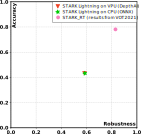
\includegraphics[width=0.8\textwidth]{img/vot_ar_plot.pdf}
    \end{center}
    \caption{Slika prikazuje retultat testa VOT-ST2021 uporabljenih sledilnikov. Graf prikazuje povprečno natančnost v odvisnosti od povprečne robustnosti. Rezultati sledilnika STARK\_RT so povzeti iz \cite{vot2021}.}
    \label{img:vot_ar}
\end{figure}

\begin{figure}[htb]
    \begin{center}
        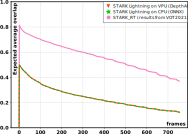
\includegraphics[width=1\textwidth]{img/vot_frames.pdf}
    \end{center}
    \caption{Slika prikazuje retultat testa VOT-ST2021 uporabljenih sledilnikov. Graf prikazuje pričakovano povprečno prekrivanje omejitvenih okvirjev skozi čas. Rezultati sledilnika STARK\_RT so povzeti iz \cite{vot2021}.}
    \label{img:vot_frames}
\end{figure}

\chapter{Zaključek}
V diplomskem delu smo implementirali in ovrednotili delovanje modernega vizualnega sledilnika STARK. Sledilnik deluje na osnovi umetnih nevronskih mrež, bolj natančno umethinh nevronskih mrež z arhitekjturo transformer. Med pregledom objavljenih del na temo vizualnega sledenja na vrgajenih napravah nismo našli nobenega, ki bi uporabil sledilnika z najmodrenejšo arhitekturo - transformer. Cilj dela je bil preučiti možnosti take implementacije, sama implementacija ter ovrednotenje delovanja sledilnika. Sledilnik smo impmementirali na vgrjanei napravi Luxonis OAK-1, ki podpira ekosistem DepthAI. Zaradi omejene procesorske moči smo se odločili za uporabo poenostavljene različice modela STARK - STARK Lightning. Sledilnik je bilo najprej potrebno predelati, ga pretvoriti v ONNX format ter ga s pomočjo nabora orodji OpenVINO optimizirati in prevesti v binarno obliko. V okolju DepthAI je bilo potrbno zasnovati cevovod, ter vanga vmestiti model. Za testiranje sledilnika smo uporabili testni nabor podatkov VOT-ST2021. Rezultati testiranja so pokazali, da je implementacija na vgrajeni napravi enaka tisti v okolju ONNX Runtime.

Implemetirali smo 4 različne načine delovanja, ki so podrobneje opisani v \ref{sec:pipeline}. Način delovanja, ki bi bil najbolj uporaben v realnem svetu \ref{sec:edge_cam}, uporabniku v realnem času prikazuje sliko, ki jo zajema kamera. Uporabnik lahko na sliki označi željeno tarčo, sledilnik pa bo tej tarči začel slediti in okoli nje izrisovati omejitveni okvir. Uporabnik lahko v bilokaterem trenutku označi novo tarčo za sledenje.

Največja slabost naše implementacije je hitrost delovanja. Sledilnik deluje z povprečno 10 FPS, kar je premalo, da bi ga lahko uvrstili med sledilnike, ki delujejo v realnem času. Ugotovili smo, da je ozko grlo v sistemu ravno napovedovanje z nevronsko mrežo, saj v povprečju traja kar 68 ms, vse ostalo procesiranje pa doprinese se 30ms. V tej smeri je odrpto še veliko možnosti za optimizacijo in predelave modela, ki bi lahko skrajšalo čas izvajanja.

%\cleardoublepage
%\addcontentsline{toc}{chapter}{Literatura}

% \printbibliography[heading=bibintoc,type=article,title={Članki v revijah}]
% https://www.overleaf.com/project/609ce2055f917cb2f776732e
% \printbibliography[heading=bibintoc,type=inproceedings,title={Članki v zbornikih}]

% \printbibliography[heading=bibintoc,type=incollection,title={Poglavja v knjigah}]

\printbibliography[heading=bibintoc,title={Celotna literatura}]


\end{document}

